\chapter{二分图中的极大二分团枚举问题}
\label{ch:intro}

二分图是图论中一种基本结构,被广泛应用于社交网络分析、推荐系统、生物信息学等领域。在二分图中,极大二分团是特殊的子图,用于描述不同群体之间的连接关系,具有重要的研究价值和应用潜力。极大二分团枚举问题在数据挖掘和图论领域中扮演着重要角色,帮助我们理解图的结构和特征,并挖掘有用的信息。例如,在电子商务中,极大二分团可以描述同时购买某批商品的用户群体,通过枚举极大二分团,可以提高对刷单行为的检测率。然而,随着二分图规模的增大,极大二分团的数量也不断增加,如何高效地进行枚举成为一个严峻挑战。本章首先概述二分图中极大二分团枚举问题的定义,随后介绍基于集合枚举树进行极大二分团枚举的基本方法,最后讨论现有方法存在的问题和挑战。

% 二分图是图论中的一种基本结构,广泛应用于许多领域,如社交网络分析、推荐系统、生物信息学等。在二分图中,极大二分团是一种特殊的子图,用来最大程度地描述两个不同群体间的连接关系,具有重要的研究价值和应用潜力。二分图中的极大二分团枚举问题在数据挖掘领域和图论领域中扮演着重要的角色,因为他可以帮助我们更好的理解图的结构和特征,进而从中挖掘有用的信息。例如,在电子商务场景中,极大二分团描述同一批用户同时购买了同一批商品。通过对极大二分团的枚举,便于找到可以交易,提升对刷单行为的检出率。随着大数据时代的到来,二分图的规模不断扩大,极大二分团的数量不断增多,在短时间内完成极大二分团枚举的计算成为了一个严峻的挑战。本章给出了二分图中的极大二分团枚举问题的概述,包括问题定义以及现有方法存在的问题与挑战。

\section{问题定义}

在问题定义之前,我们首先介绍图论领域的一些基础概念,并提供了随后频繁使用的符号及其含义,如~\autoref{tab:definition}所示。

\begin{longtable}[htbp]{|c|p{12cm}|}
    \caption{本文使用的符号及含义}
    \label{tab:definition} \\
    
    \hline
    符号 & 含义 \\ \hline
    \endfirsthead
    
    \hline
    符号 & 含义 \\ \hline
    \endhead
    
    \hline
    \multicolumn{2}{r}{续下页} \\
    \endfoot
    
    \hline
    \endlastfoot
    
    $G(U,V,E)$ & 一个无向二分图 $G$,其中 $U$ 和 $V$ 是两个不相交的顶点集合,$E$ 是二分图的边集合且 $E \subseteq U \times V$。 \\ \hline
    $u,v$ & 表示二分图 $G$ 中的顶点。其中顶点 $u$ 属于集合 $U$,顶点 $v$ 属于集合 $V$。 \\ \hline
    $N(v)$ & 表示顶点 $v$ 的邻居顶点集合,即 $N(v) = \{u \,|\, (u,v) \in E\}$。 \\ \hline
    $N_2(v)$ & 表示顶点 $v$ 的二跳邻居顶点集合,即 $N_2(v) = \bigcup_{u \in N(v)} N(u) - \{v\}$。 \\ \hline
    $\Gamma(X)$ & 表示顶点集 $X$ 内顶点的共同邻居,即 $\Gamma(X) = \bigcap_{v \in X} N(v)$。 \\ \hline
    $\Delta(X)$ & 表示顶点集 $X$ 内顶点的最大度数,即 $\Delta(X) = \max_{u \in X} |N(u)|$。 \\ \hline
    $\Delta_2(X)$ & 表示顶点集 $X$ 内顶点的最大二跳度数,即 $\Delta_2(X) = \max_{u \in X} |N_2(u)|$。 \\ \hline
    $X_v^+, X_v^-$ & 表示顶点集 $X$ 根据顶点 $v$ 划分成的两个子集。给定一个顶点顺序,$X_v^+$ 包含所有顶点比 $v$ 更大的顶点(顺序在 $v$ 之后的顶点);$X_v^-$ 包含包括 $v$ 顶点在内的所有顶点比 $v$ 更小的顶点(顺序在 $v$ 之前的顶点)。 \\ \hline
    $L,R,C$ & $L$, $R$ 和 $C$ 指三个两两不相交的顶点集,其中 $L$ 是 $U$ 集合的子集,$R$ 和 $C$ 是 $V$ 集合的子集。$L,R$ 和 $C$ 共同构成一个枚举树节点,其中 $(L,R)$ 表示枚举树节点对应的二分团,$C$ 表示用于产生新枚举树节点的候选顶点。对于二分团 $(L,R)$,$L$ 和 $R$ 分别表示二分团的左部顶点集和右部顶点集。 \\ \hline
    $N_L(v)$ & 表示顶点 $v$ 的局部邻居。对于对应二分团 $(L,R)$ 的枚举树节点,$N_L(v) = L \cap N(v)$。 \\ \hline
    $\vec{v}$ & 对于一个枚举树节点,$v$ 表示用于生成该枚举树节点的候选顶点。 \\ \hline
    $\alpha, \delta, \beta$ & 对于一棵极大二分团枚举树,$\alpha$ 表示枚举树中产生的极大二分团的数量,$\delta$ 表示枚举树中产生的其他二分团的数量,$\beta$ 表示枚举树中二分团的总数量。可知 $\beta = \alpha + \delta$。 \\ \hline
\end{longtable}

  二分图中的极大二分团枚举问题是在一个无向二分图$G(U,V,E)$中的子图挖掘问题。随后,我们正式定义二分团、极大二分团以及极大二分团枚举问题。

\begin{definition}
  \textup{\textbf{(二分团)}} 二分团(biclique)是二分图$G(U,V,E)$中的稠密二分子图$(L,R,E')$。其中$L\subseteq U$, $R\subseteq V$, $E' = L \times R \subseteq E$。为了方便,下文中我们直接用顶点集对$(L,R)$表示二分团。
\end{definition}

\begin{definition}
  \textup{\textbf{(极大二分团)}} 极大二分团(maximal biclique)是二分图$G$中的一个二分团,且该二分团不能再添加其他顶点使其成为更大的二分团。
\end{definition}

\begin{definition}
  \textup{\textbf{(极大二分团枚举问题)}} 极大二分团枚举问题(maximal biclique enumeration)的目标是无重复、无遗漏地枚举枚举二分图中的全部极大二分团。
\end{definition}

\begin{figure} [ht]
  \vspace{0.1 in}
  \centering
  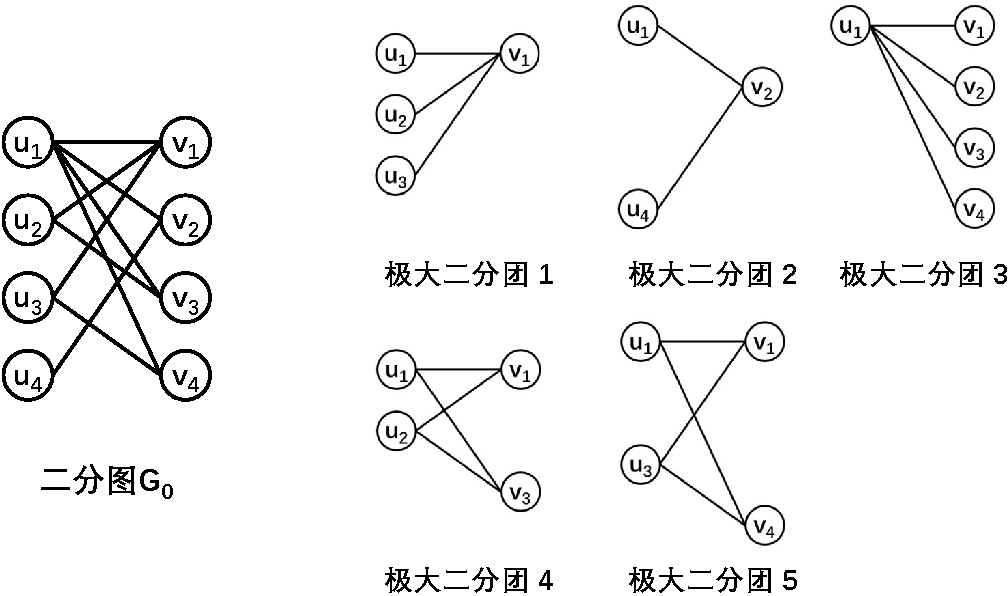
\includegraphics[width=0.6\linewidth]{eg_definition}
  \vspace{0.1 in}
  \caption{二分图中的极大二分团枚举问题示例}
  \label{fig:eg_definition}
\end{figure}

\begin{example}
  ~\autoref{fig:eg_definition}给出了一个二分图中的极大二分团枚举问题的示例。其中左图是一个具有9个顶点,12条边的二分图$G_0$,右图展示了二分图中的全部极大二分团,共6个。
  
\end{example}


\section{存在的问题与挑战}

